%%%%%%%%%%%%%%%%%%%%%%%%%%%%%%% main.tex %%%%%%%%%%%%%%%%%%%%%%%%%%%%%%%
%                                                                      %
% --------------------- Report Template IST [EN] --------------------- %
%                                                                      %
%       João Marafuz Gaspar                                            %
%       Departamento de Engenharia Eletrotécnica e de Computadores     %
%       Instituto Superior Tecnico                                     %
%       Av. Rovisco Pais                                               %
%       1049-001 Lisboa                                                %
%       Portugal                                                       %
%       E-mail: joao.marafuz.gaspar@tecnico.ulisboa.pt                 %
%                                                                      %
%  Created:       Jul 30, 2022                                         %
%  Last Modified: Jul 30, 2022                                         %
%                                                                      %
%%%%%%%%%%%%%%%%%%%%%%%%%%%%%%%%%%%%%%%%%%%%%%%%%%%%%%%%%%%%%%%%%%%%%%%%
%  Revision history                                                    %
%  v1 - 2022/07/30 - original template                                 %
%%%%%%%%%%%%%%%%%%%%%%%%%%%%%%%%%%%%%%%%%%%%%%%%%%%%%%%%%%%%%%%%%%%%%%%%
%                              Preamble                                %
%%%%%%%%%%%%%%%%%%%%%%%%%%%%%%%%%%%%%%%%%%%%%%%%%%%%%%%%%%%%%%%%%%%%%%%%

% ----------------------------------------------------------------------
% Set the document class
% ----------------------------------------------------------------------
\documentclass[12pt]{article}

% ----------------------------------------------------------------------
% Define external packages, language, margins, fonts, new commands 
% and colors
% ----------------------------------------------------------------------
\usepackage[utf8]{inputenc} % Codification
\usepackage[english]{babel} % Writing idiom

\usepackage[export]{adjustbox} % Align images
\usepackage{amsmath} % Extra commands for math mode
\usepackage{amssymb} % Mathematical symbols
\usepackage{amsthm}
\usepackage{anysize} % Personalize margins
    \marginsize{2cm}{2cm}{2cm}{2cm} % {left}{right}{above}{below}
\usepackage{appendix} % Appendices
\usepackage{cancel} % Expression cancellation
\usepackage{caption} % Figure numeration
\usepackage{cite} % Citations, like [1 - 3]
\usepackage{color} % Text coloring
\usepackage{fancyhdr} % Head note and footnote
    \pagestyle{fancy}
    \fancyhf{}
    \fancyhead[L]{\footnotesize IST} % Left of Head note
    \fancyhead[R]{\footnotesize ULisboa} % Right of Head note
    %\fancyfoot[L]{\footnotesize Course} % Left of Footnote
    \fancyfoot[C]{\thepage} % Center of Footnote
    %\fancyfoot[R]{\footnotesize Degree} % Right of Footnote
    \renewcommand{\footrulewidth}{0.4pt} % Footnote rule
\usepackage{float} % Utilization of [H] in figures
\usepackage{graphicx} % Figures in LaTeX
\usepackage[colorlinks = true, plainpages = true, linkcolor = istblue, urlcolor = istblue, citecolor = istblue, anchorcolor = istblue]{hyperref}
\usepackage{indentfirst} % First paragraph
\usepackage{siunitx} % SI units
\usepackage{subfigure} % Subfigures

% Random text (not needed)
\usepackage{lipsum}
\usepackage{duckuments}

% New and re-newcommands
\newcommand{\sen}{\operatorname{\sen}} % Sine function definition
\newcommand{\HRule}{\rule{\linewidth}{0.5mm}} % Specific rule definition
\renewcommand{\appendixpagename}{\LARGE Appendices}

% Colors
\definecolor{istblue}{RGB}{3, 171, 230}
\definecolor{dkgreen}{rgb}{0,0.6,0}
\definecolor{gray}{rgb}{0.5,0.5,0.5}

%%%%%%%%%%%%%%%%%%%%%%%%%%%%%%%%%%%%%%%%%%%%%%%%%%%%%%%%%%%%%%%%%%%%%%%%
%                                 Document                             %
%%%%%%%%%%%%%%%%%%%%%%%%%%%%%%%%%%%%%%%%%%%%%%%%%%%%%%%%%%%%%%%%%%%%%%%%
\begin{document}

% ----------------------------------------------------------------------
% Cover
% ----------------------------------------------------------------------
\begin{center}
    \begin{figure}
        \vspace{-1.0cm}
        
\includegraphics[scale = 0.3, left]{Images/IST_A.eps} % IST logo
    \end{figure}
    \mbox{}\\[2.0cm]
    \textsc{\Huge Optimization and Algorithms Project}\\[2.5cm]
    %\textsc{\LARGE Degree}\\[2.0cm]
    %\HRule\\[0.4cm]
    %{\large \bf Title -- Report Template IST [\texttt{EN}]}\\[0.2cm]
    %\HRule\\[1.5cm]
\end{center}

\begin{flushleft}
    \textbf{Authors:}
\end{flushleft}

\begin{center}
    \begin{minipage}{0.5\textwidth}
        \begin{flushleft}
            Duarte Calado de Almeida (95565)\\
            Francisco Manuel Leal Mitha Ribeiro (95578)\\
            João De Assis Marcos Soares Nabais (97349)\\ 
            João De Assis Marcos Soares Nabais (965259)
        \end{flushleft}
    \end{minipage}%
    %\begin{minipage}{0.5\textwidth}
    %    \begin{flushright}
    %        \href{mailto:joao.marafuz.gaspar@tecnico.ulisboa.pt}{\texttt{joao.marafuz.gaspar@tecnico.ulisboa.pt}}\\
    %        \href{mailto:lorem.ipsum@tecnico.ulisboa.pt}{\texttt{lorem.ipsum@tecnico.ulisboa.pt}}\\
    %        \href{mailto:lorem.ipsum@tecnico.ulisboa.pt}{\texttt{lorem.ipsum@tecnico.ulisboa.pt}}
    %    \end{flushright}
    %\end{minipage}
\end{center}
    
\begin{flushleft}
    \large $\boxed{\text{\bf Group} \ 8}$\\[4.0cm]
\end{flushleft}
    
\begin{center}
    \large \bf 2022/2023 -- 1º Semester, P1
\end{center}

\thispagestyle{empty}

\setcounter{page}{0}

\newpage

% ----------------------------------------------------------------------
% Contents
% ----------------------------------------------------------------------
\tableofcontents 

\newpage

% ----------------------------------------------------------------------
% Body
% ----------------------------------------------------------------------
\section{Task 1}

\begin{figure}[H]
    \centering
    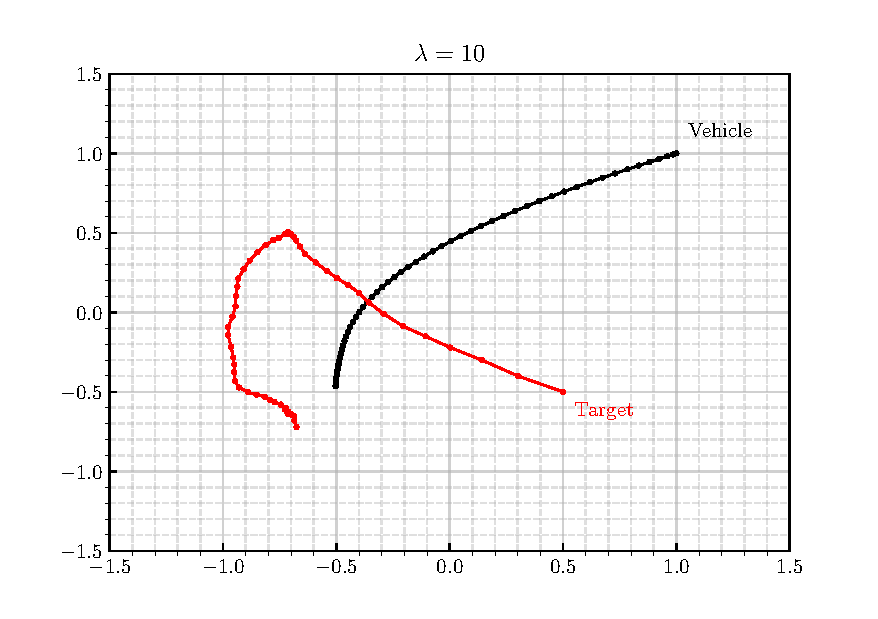
\includegraphics{../../src/task_1/output/ex_1_i=1.pdf}
\end{figure}

\begin{figure}[H]
    \centering
    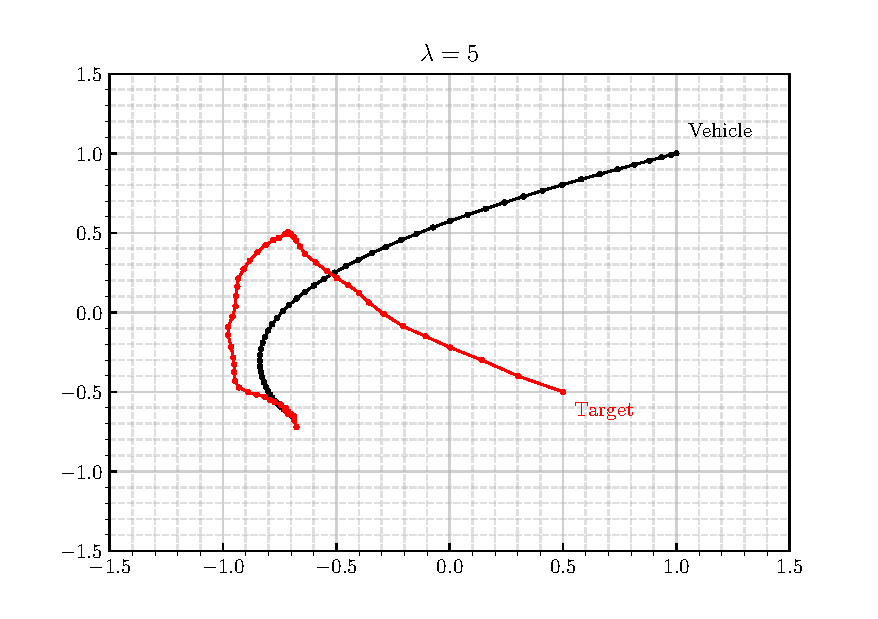
\includegraphics{../../src/task_1/output/ex_1_i=2.pdf}
\end{figure}

\begin{figure}[H]
    \centering
    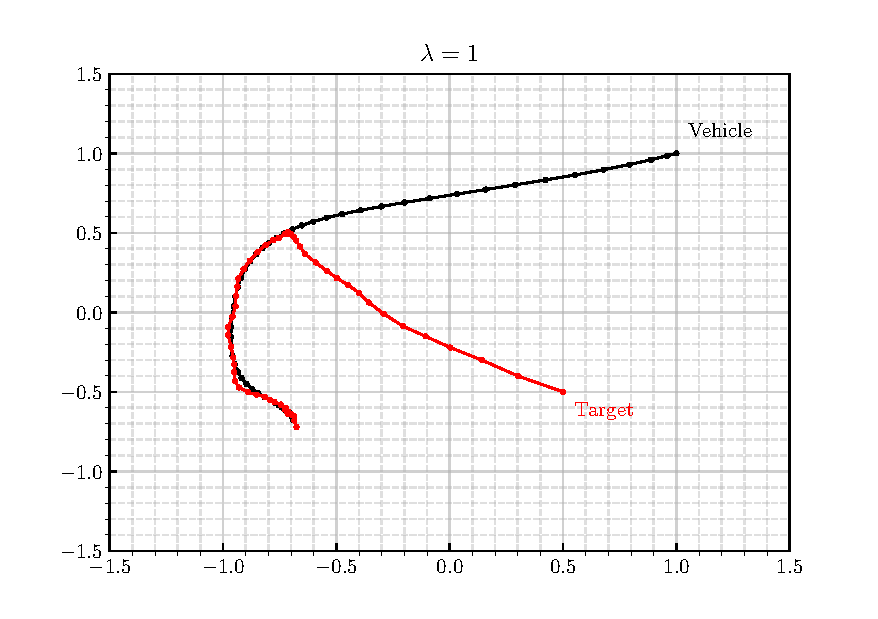
\includegraphics{../../src/task_1/output/ex_1_i=3.pdf}
\end{figure}

\begin{figure}[H]
    \centering
    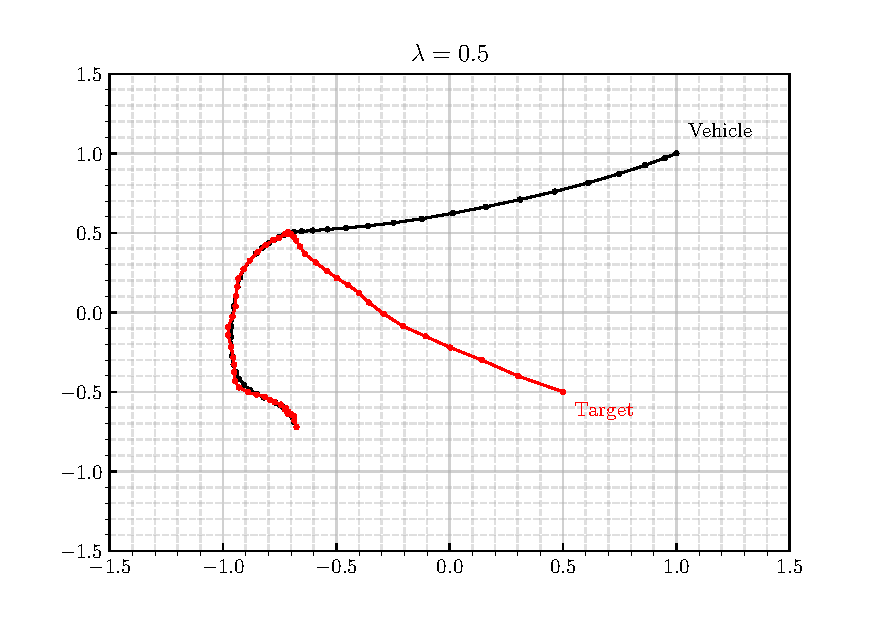
\includegraphics{../../src/task_1/output/ex_1_i=4.pdf}
\end{figure}

\begin{figure}[H]
    \centering
    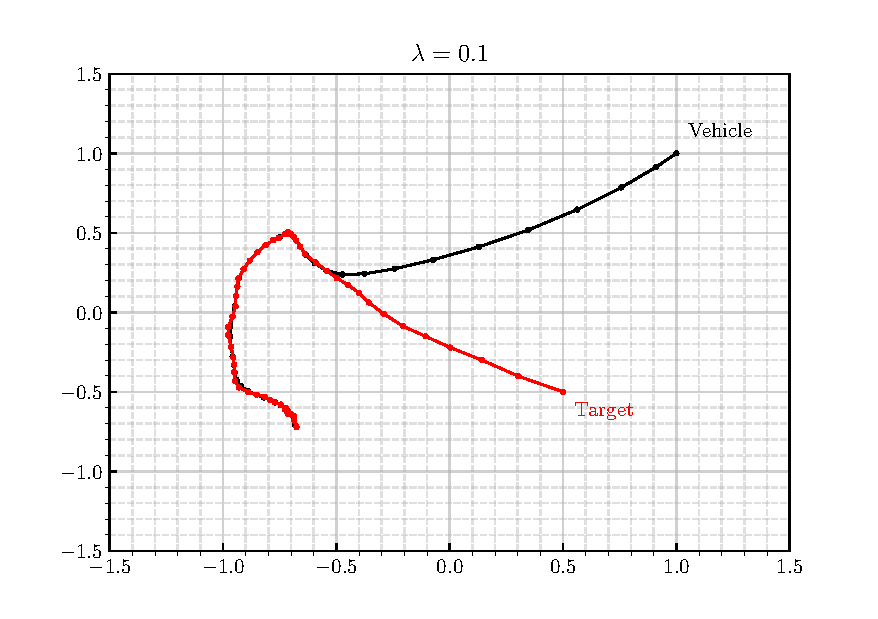
\includegraphics{../../src/task_1/output/ex_1_i=5.pdf}
\end{figure}

\begin{figure}[H]
    \centering
    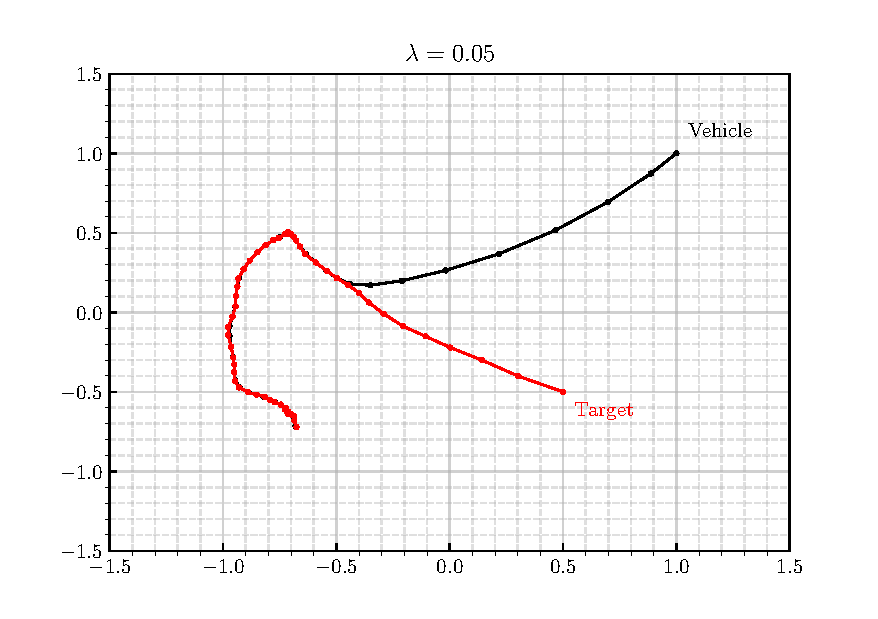
\includegraphics{../../src/task_1/output/ex_1_i=6.pdf}
\end{figure}

\begin{figure}[H]
    \centering
    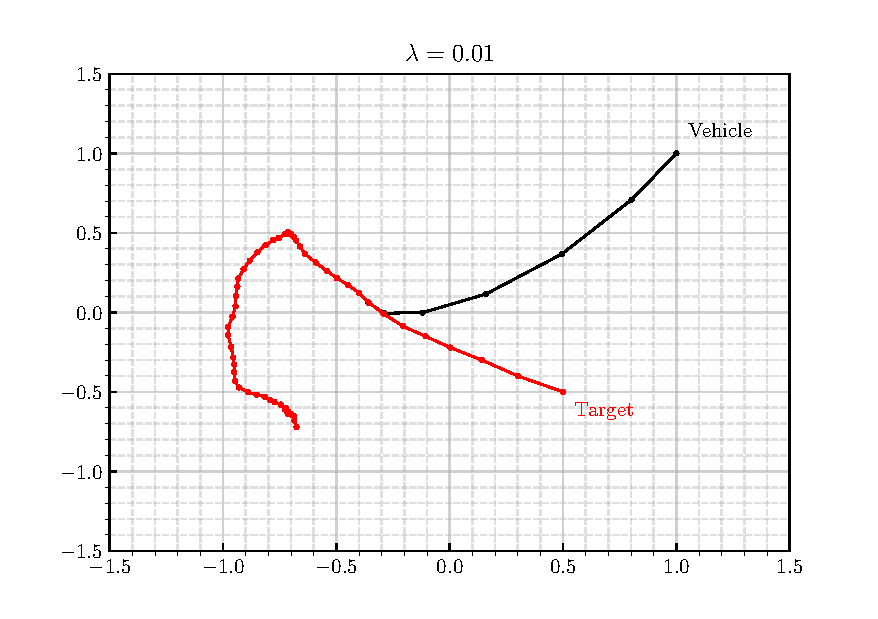
\includegraphics{../../src/task_1/output/ex_1_i=7.pdf}
\end{figure}

\begin{figure}[H]
    \centering
    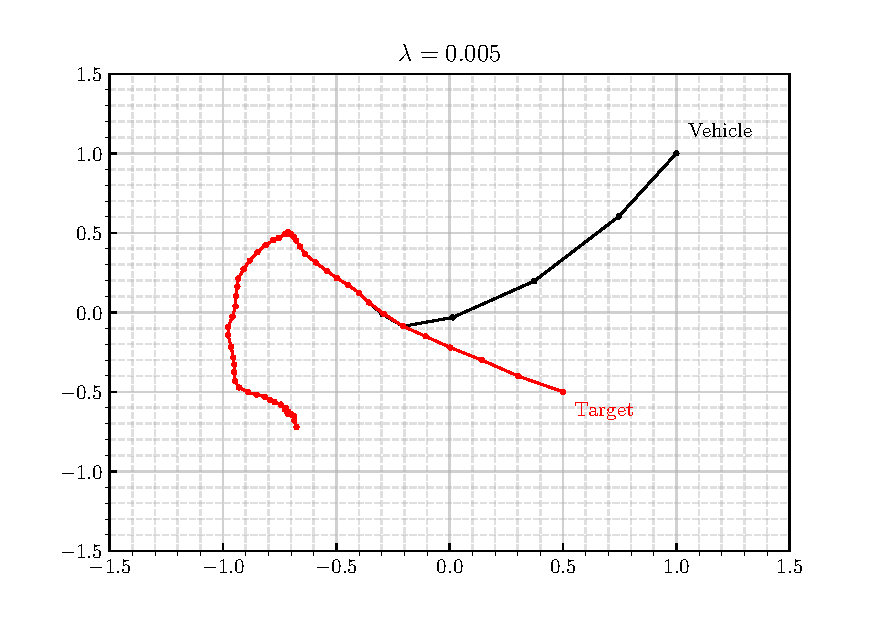
\includegraphics{../../src/task_1/output/ex_1_i=8.pdf}
\end{figure}

\begin{figure}[H]
    \centering
    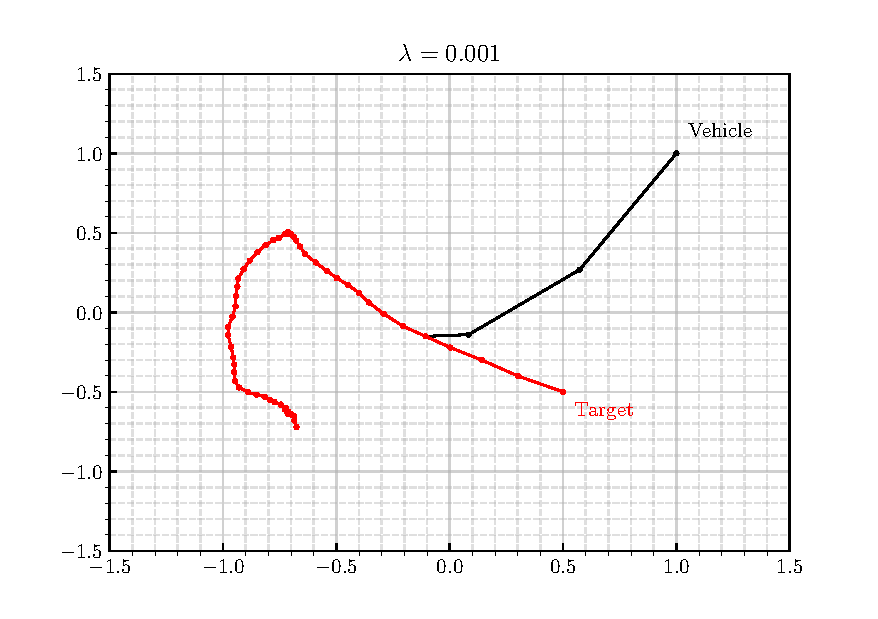
\includegraphics{../../src/task_1/output/ex_1_i=9.pdf}
\end{figure}

\begin{figure}[H]
    \centering
    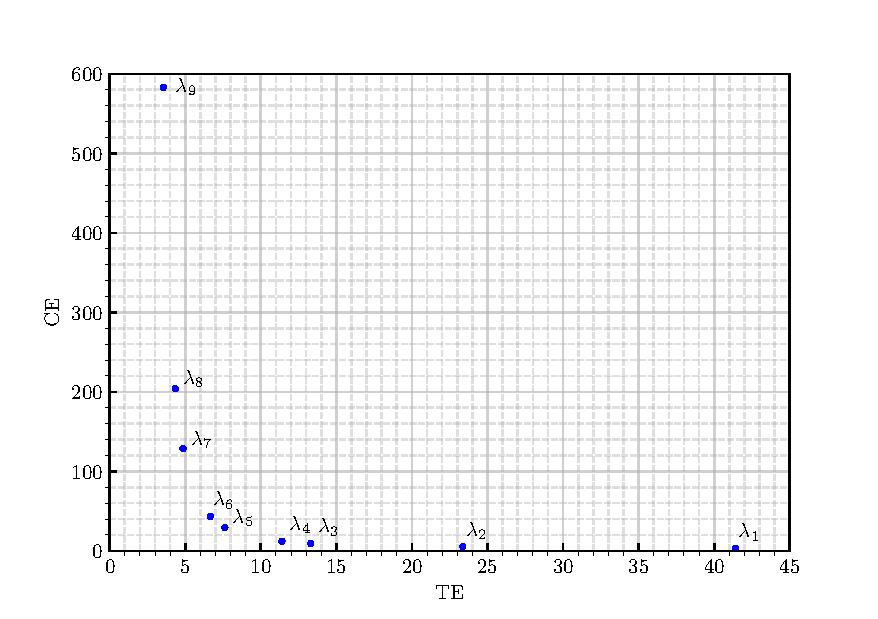
\includegraphics{../../src/task_1/output/TEvsCE.pdf}
\end{figure}

When the parameter $\lambda$ increases, the Tracking and Control Efforts associated with the optimal solution of the resulting optimization problem increases and decreases, respectively. \\

\section{Task 2}

\begin{proof}[\unskip\nopunct]
    Let $(x_a, u_a)$ and $(x_b, u_b)$ denote the minimizers obtained after solving the given optimization problem for $\lambda = \lambda_{a}$ and $\lambda = \lambda_{b}$, respectively. Let $\text{TE}(x, u)$ and $\text{CE}(x, u)$ denote the Tracking and Control Efforts for a given value of $(x, u) = (x(1), ..., x(T), u(1), ..., u(T - 1))$, respectively.
    Then, suppose that $\text{TE}(x_a, u_a) \le \text{TE}(x_b, u_b)$.

    Since $(x_b, u_b)$ minimizes the given optimization problem for $\lambda = \lambda_b$, it follows that:
    \vspace{-0.3em}
    \begin{align}
        \text{TE}(x_b, u_b) + \lambda_b \text{CE}(x_b, u_b) & \le 
        \text{TE}(x_a, u_a) + \lambda_b \text{CE}(x_a, u_a) \\
        & = 
        \text{TE}(x_a, u_a) + \lambda_a \text{CE}(x_a, u_a) + ( \lambda_b -  \lambda_a) \text{CE}(x_a, u_a) \\
        & \le 
        \text{TE}(x_b, u_b) + \lambda_a \text{CE}(x_a, u_a) + ( \lambda_b -  \lambda_a) \text{CE}(x_a, u_a) \\
        & = \text{TE}(x_b, u_b) + \lambda_b \text{CE}(x_a, u_a)
    \end{align}

    where we used the hypothesis that $\text{TE}(x_a, u_a) \le \text{TE}(x_b, u_b)$ do derive (3) from (2). In particular, we have that:
    \vspace{-0.3em}
    \begin{align}
        \text{TE}(x_b, u_b) + \lambda_b \text{CE}(x_b, u_b) & \le 
        \text{TE}(x_b, u_b) + \lambda_b \text{CE}(x_a, u_a) \\
        \Leftrightarrow \lambda_b \text{CE}(x_b, u_b) & \le 
        \lambda_b \text{CE}(x_a, u_a) \\
        \Leftrightarrow \text{CE}(x_b, u_b) &\le \text{CE}(x_a, u_a)
    \end{align}

    with the last inequality coming from the fact that $\lambda_b > 0$. We have thus proven the desired result.
\end{proof}







\appendix  
\clearpage
\addappheadtotoc 
\appendixpage 

\section{First appendix}

\lipsum[1]

\section{Second appendix}

\lipsum[1]
\end{document}